\documentclass[conference]{IEEEtran}

\usepackage{hyperref}



% *** GRAPHICS RELATED PACKAGES ***
%
\ifCLASSINFOpdf
  \usepackage[pdftex]{graphicx}
  % declare the path(s) where your graphic files are
  \graphicspath{ {pictures/}{../pdf/}{../jpeg/} }
  % and their extensions so you won't have to specify these with
  % every instance of \includegraphics
  \DeclareGraphicsExtensions{.pdf,.jpeg,.png,.PNG}
\else
 
\fi


\usepackage{amsmath}





% *** SUBFig PACKAGES ***
\ifCLASSOPTIONcompsoc
 \usepackage[caption=false,font=normalsize,labelfont=sf,textfont=sf]{subfig}
\else
 \usepackage[caption=false,font=footnotesize]{subfig}
\fi



% correct bad hyphenation here
\hyphenation{op-tical net-works semi-conduc-tor}


% ------ Spencer's Adds: -----------
% HOW TO make a command ("tab" here)
\newcommand\tab[1][0.4cm]{\hspace*{#1}}
% This line makes the collumns on the last line even
\usepackage{flushend}
\usepackage{tabularx,booktabs,textcomp}
% Additions for custom TabularX environment tables: 
\newcolumntype{C}{>{\centering\arraybackslash}X} % centered version of "X" type
\newcolumntype{L}{>{\raggedright\arraybackslash}X} % LEFT version... "\...right" works?
% Next three lines take [1], [2], [3], [4] and cite as [1-4]:
\usepackage[noadjust]{cite}
\renewcommand{\citepunct}{,\penalty\citepunctpenalty\,}
\renewcommand{\citedash}{--}    % optionally
% Include Smileys :) 
\usepackage{wasysym}
% Include to generate random text: 
\usepackage{lipsum} % USE: "\lipsum[1]" to generate 1 paragraph of random text 
% ----------------------------------

\begin{document}

\title{Title}

% AUTHOR
\author{\IEEEauthorblockN{Author Name, matriculation number}
\IEEEauthorblockA{Programme of Study\\
University of Edinburgh\\
}}

% make the title area
\maketitle

% As a general rule, do not put math, special symbols or citations
% in the abstract
\begin{abstract}

These instructions give you guidelines for preparing papers for your ERMGC coursework using a template that is adapted from IEEE Transactions and Journals. Use this document as a template if you are using \LaTeX. Paper titles should be written in uppercase and lowercase letters, not all uppercase. Avoid writing long formulas with subscripts in the title; short formulas that identify the elements are fine (e.g., "Nd–Fe–B"). The abstract must be a concise yet comprehensive reflection of what is in your article. In particular, the abstract must be self-contained, without abbreviations, footnotes, or references. It should be a microcosm of the full article. The abstract must be between 150–250 words. The abstract must be written as one paragraph, and should not contain displayed mathematical equations or tabular material. The abstract should include three or four different keywords or phrases, as this will help readers to find it. It is important to avoid over-repetition of such phrases as this can result in a page being rejected by search engines. Ensure that your abstract reads well and is grammatically correct.\\
\end{abstract}
% no keywords

\begin{IEEEkeywords}
Enter key words or phrases in alphabetical order, separated by commas. 
\end{IEEEkeywords}


\section{Introduction}

Example of citations: \cite{Chen1993Linear} and \cite{farrar2007introduction, movsessian2021artificial}. This document is a template for \LaTeX. It is recommended to use \url{https://www.overleaf.com/}. If you log in with you University of Edinburgh email, you should have access to the professional version in overleaf.




\section{Guidelines for manuscript preparation}
\label{sec:op}

Do not change the font sizes or line spacing to squeeze more text into a limited number of pages. Use italics for emphasis; do not underline


\subsection{Abbreviations and Acronyms}

Define abbreviations and acronyms the first time they are used in the text, even after they have already been defined in the abstract. Abbreviations such as IEEE, SI, ac, and dc do not have to be defined. Abbreviations that incorporate periods should not have spaces: write “C.N.R.S.,” not “C. N. R. S.” Do not use abbreviations in the title unless they are unavoidable.

\subsection{Other Recommendations}

Use one space after periods and colons. Hyphenate complex modifiers: “zero-field-cooled magnetization.” Avoid dangling participles, such as, “Using (\ref{eq:1}) the energy was calculated.” [It is not clear who or what used (\ref{eq:1}).] Write instead, “The energy was calculated by using (\ref{eq:1}),” or “Using (\ref{eq:1}), we calculated the energy.”



A parenthetical statement at the end of a sentence is punctuated outside of the closing parenthesis (like this). (A parenthetical sentence is punctuated within the parentheses.) 

If you wish, you may write in the first person singular or plural and use the active voice (“I observed that ...” or “We observed that ...” instead of “It was observed that ...”). Remember to check spelling. 


\section{Math}

Number equations consecutively with equation numbers in parentheses flush with the right margin, as in (\ref{eq:1}). First use the equation editor to create the equation. Use parentheses to avoid ambiguities in denominators. Punctuate equations when they are part of a sentence, as in (\ref{eq:1})

\begin{equation}
    \label{eq:1}
    A=B-C
\end{equation}
%
where $B$ and $C$ are the input the system, respectively. 

Be sure that the symbols in your equation have been defined before the equation appears or immediately following. Italicize symbols (T might refer to temperature, but T is the unit tesla). Refer to “(\ref{eq:1})),” not “Eq. (\ref{eq:1})” or “equation (\ref{eq:1})),” except at the beginning of a sentence: “Equation (\ref{eq:1}) is ... .” 


\section{Units}

Use either SI (MKS) or CGS as primary units. (SI units are strongly encouraged.) English units may be used as secondary units (in parentheses). This applies to papers in data storage. For example, write “15 Gb/cm2 (100 Gb/in$^2$).” Avoid combining SI and CGS units, such as current in amperes and magnetic field in oersteds. This often leads to confusion because equations do not balance dimensionally. If you must use mixed units, clearly state the units for each quantity in an equation. The SI unit for magnetic field strength H is A/m. 

\section{Some common Mistakes}

The word “data” is plural, not singular. The subscript for the permeability of vacuum µ0 is zero, not a lowercase letter “o.” The term for residual magnetization is “remanence”; the adjective is “remanent”; do not write “remnance” or “remnant.” Use the word “micrometer” instead of “micron.” A graph within a graph is an “inset,” not an “insert.” The word “alternatively” is preferred to the word “alternately” (unless you really mean something that alternates). Use the word “whereas” instead of “while” (unless you are referring to simultaneous events). Do not use the word “essentially” to mean “approximately” or “effectively.” Do not use the word “issue” as a euphemism for “problem.” 

Be aware of the different meanings of the homophones “affect” (usually a verb) and “effect” (usually a noun), “complement” and “compliment,” “discreet” and “discrete,” “principal” (e.g., “principal investigator”) and “principle” (e.g., “principle of measurement”). Do not confuse “imply” and "infer". 

Pefixes such as “non,” “sub,” “micro,” “multi,” and “ultra” are not independent words; they should be joined to the words they modify, usually without a hyphen. There is no period after the “et” in the Latin abbreviation “et al.” (it is also italicized). The abbreviation “i.e.,” means “that is,” and the abbreviation “e.g.,” means “for example” (these abbreviations are not italicized).

\section{Guidelines for graphics preparation and submission}

A typical figure representation like Fig.\ref{fig:1} and Table \ref{tb:1}.

\begin{figure}[h] % t,h, and b mean "top," "in-line," and "bottom" respectively
  \centering
  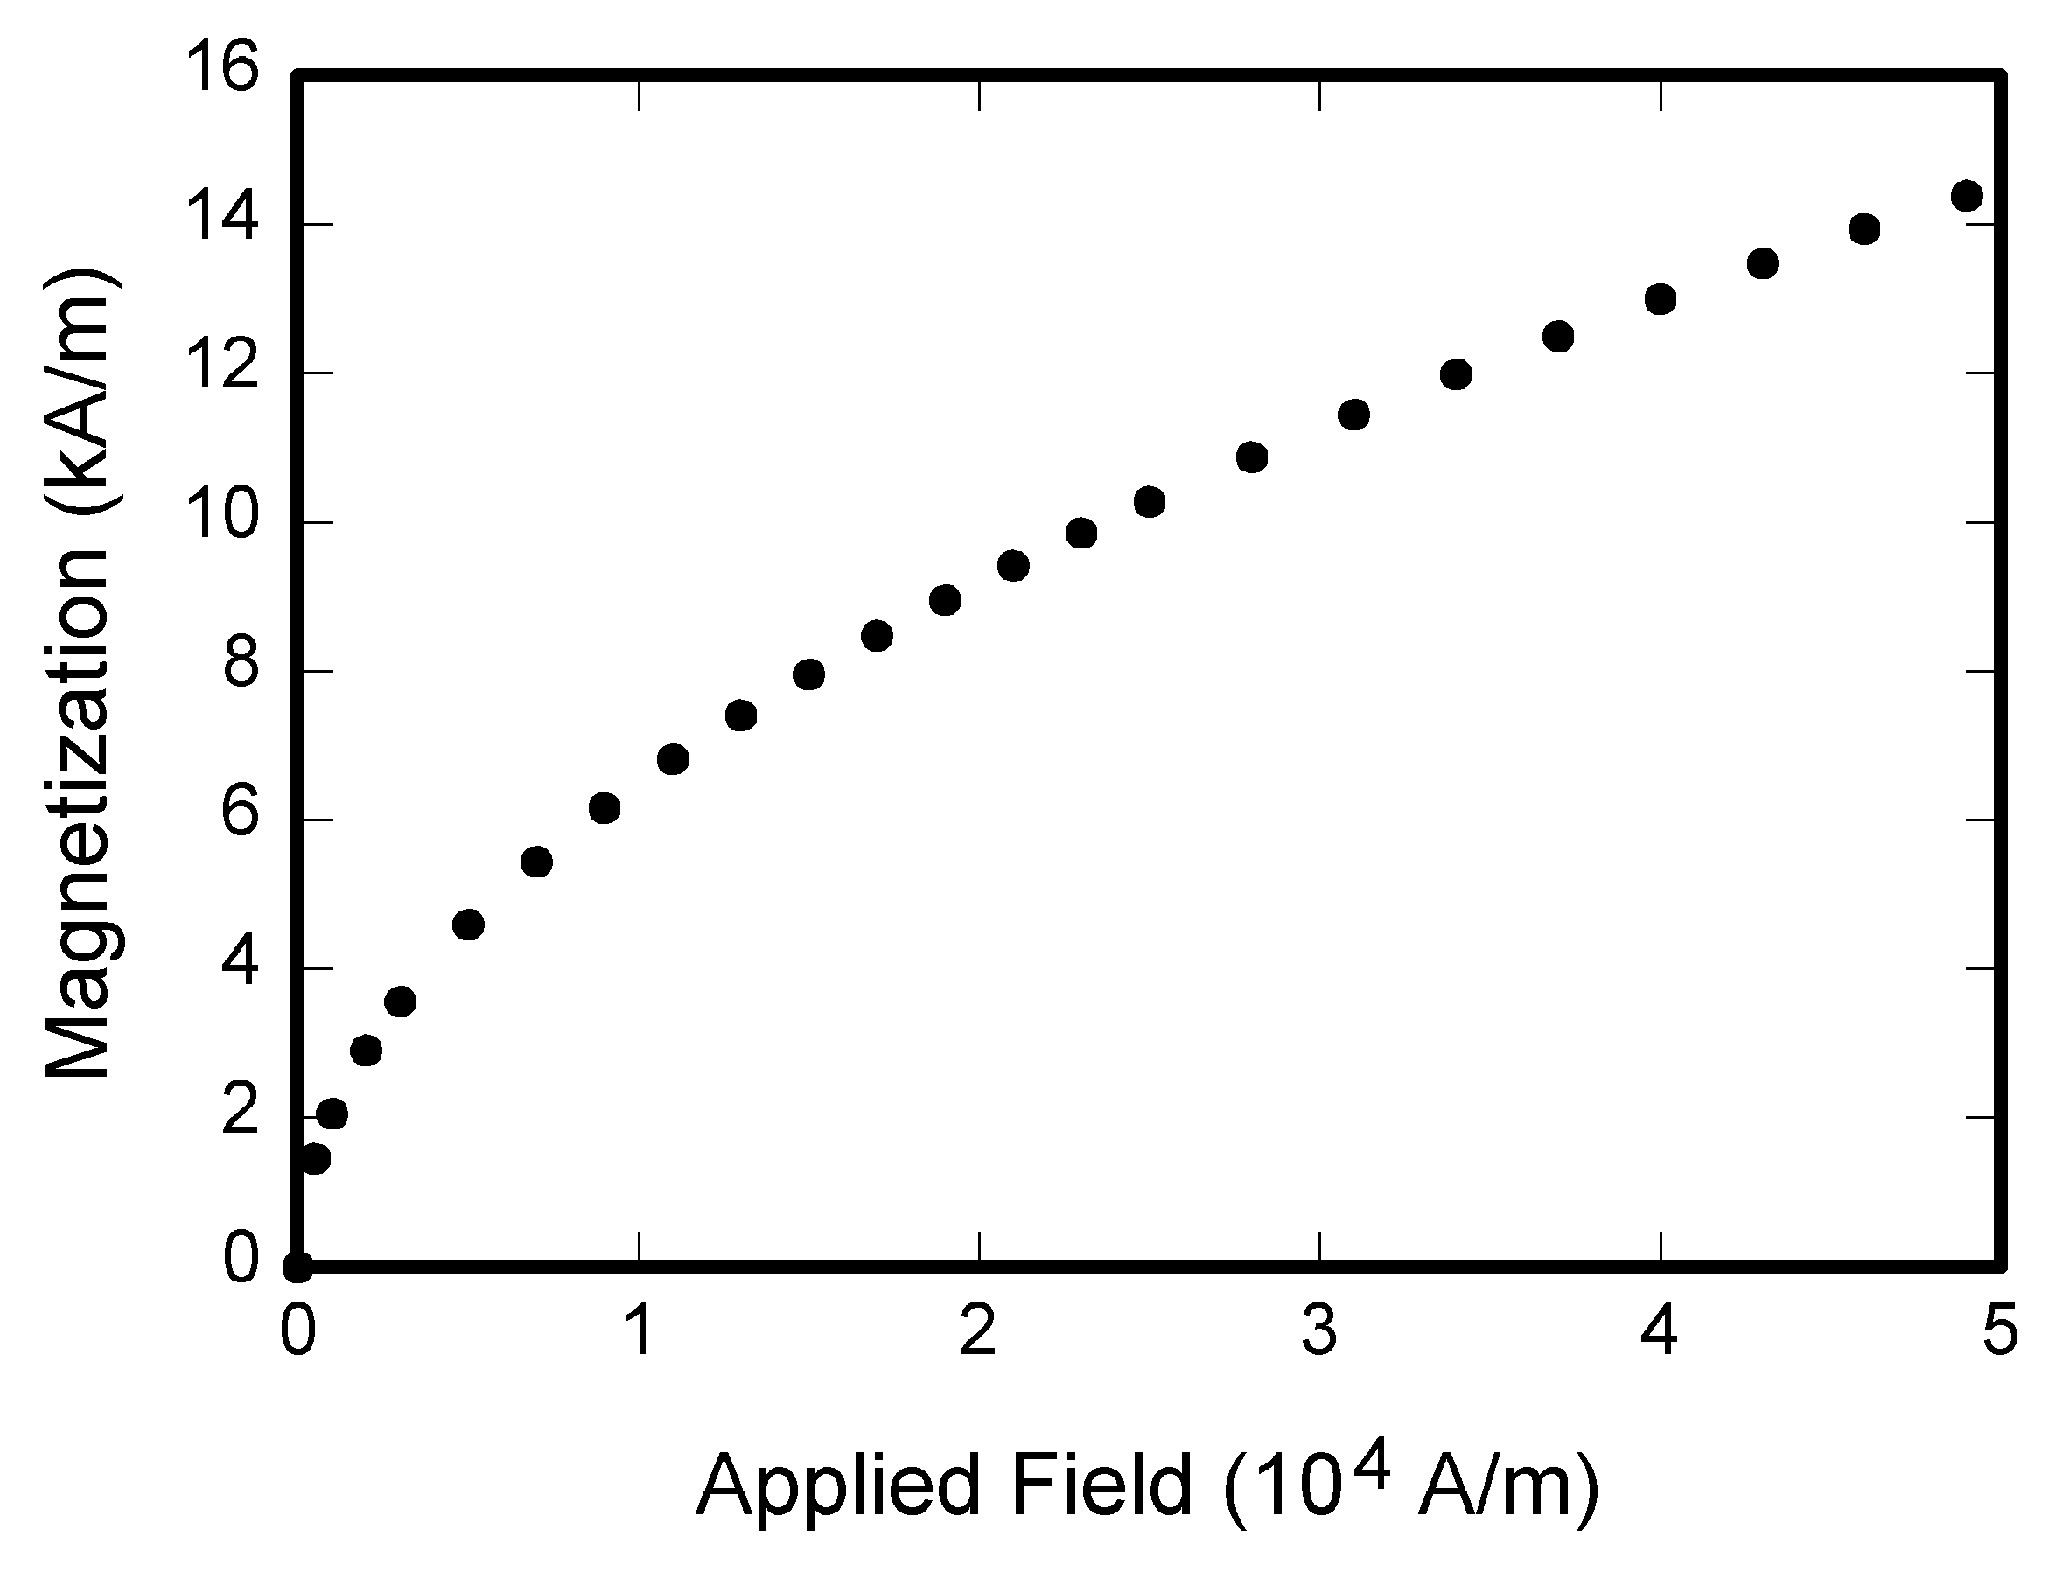
\includegraphics[width=2.8in]{pictures/Fig1.jpg}\\
  \caption{Magnetization as a function of applied field. Note that “Fig.” is abbreviated. There is a period after the figure number, followed by two spaces. It is good practice to explain the significance of the figure in the caption.}\label{fig:1}
\end{figure}



\begin{table}[ht]
\centering
\caption{Example Table}
\label{classEeffs}
\begin{tabularx}{2.7in}{C C C}
\toprule
        cell \# & Frequency & Power\\ 
\midrule
        cell1   & 5.56 MHz      & 10 W      \\
        cell2   & 6.78 MHz      & 10 W       \\
        cell3   & 6.78 MHz      & 27 W        \\

\bottomrule
\end{tabularx}
\vspace{0.5mm}\\
\label{tb:1}
\end{table}

\subsection{Sizing of Graphics} 

Most charts, graphs, and tables are one column wide (3.5 inches / 88 millimeters / 21 picas) or page wide (7.16 inches / 181 millimeters / 43 picas). The maximum depth a graphic can be is 8.5 inches (216 millimeters / 54 picas). When choosing the depth of a graphic, please allow space for a caption. Figures can be sized between column and page widths if the author chooses, however it is recommended that figures are not sized less than column width unless when necessary. 

\subsection{Using Labels Within Figures} 
\subsubsection{Figures Axis labels}

Figure axis labels are often a source of confusion. Use words rather than symbols. As an example, write the quantity “Magnetization,” or “Magnetization M,” not just “M.” Put units in parentheses. Do not label axes only with units. As in Fig. \ref{fig:1}, for example, write “Magnetization (A/m)” or “Magnetization (A m$^{-1}$),” not just “A/m.” Do not label axes with a ratio of quantities and units. For example, write “Temperature (K),” not “Temperature/K.” 
Multipliers can be especially confusing. Write “Magnetization (kA/m)” or “Magnetization (103 A/m).” Do not write “Magnetization (A/m) $\times$ 1000” because the reader would not know whether the top axis label in Fig. \ref{fig:1} meant 16000 A/m or 0.016 A/m. Figure labels should be legible, approximately 8 to 10 point type.

\subsubsection{Subfigure Labels in Multipart Figures and Tables}

Multipart figures should be combined and labeled before final submission. Labels should appear centered below each subfigure in 8 point Times New Roman font in the format of (a) (b) (c). 

\subsubsection{Referencing a Figure or Table Within Your Paper}

When referencing your figures and tables within your paper, use the abbreviation “Fig.” even at the beginning of a sentence. Do not abbreviate “Table.” Tables should be numbered with Roman Numerals.

\section{Conclusions}
\label{sec:conc}

A conclusion section is expected for the ERMGC coursework (see assignment information in Learn). Your conclusion should review the main points of the paper and should not include any new material.  It might elaborate on the importance of the work or suggest applications and extensions. Do not replicate the abstract as the conclusion.

\subsection*{Appendix}

Appendixes, if needed, appear before the acknowledgment.  You may use Appendixes if you wish, but you should be aware that markers will normally stop reading at the end of page 5 (except for checking any references that appear after the end of page 5).

\subsection*{Acknowledgements}

The preferred spelling of the word “acknowledgment” in American English is without an “e” after the “g.” Use the singular heading even if you have many acknowledgments. Avoid expressions such as “One of us (S.B.A.) would like to thank ... .” Instead, write “F. A. Author thanks ... .” 

\subsection*{References and footnotes}

References should be cited in text. For the ERMGC coursework, you can use the IEEE format described here or another recognized referencing system (e.g. Harvard, Vancouver…).  
Number footnotes separately in superscripts\footnote{It is recommended that footnotes be avoided (except for the unnumbered footnote with the receipt date on the first page). Instead, try to integrate the footnote information into the text.}.  Place the actual footnote at the bottom of the column in which it is cited; do not put footnotes in the reference list (endnotes). Use letters for table footnotes (see Table \ref{tb:1}). 

%------- CITATIONS ----------
\bibliography{references}


\bibliographystyle{IEEEtran}



% that's all folks
\end{document}


